% Micropropulsion Heater–Nozzle Model: Methods and Results
\documentclass[11pt,a4paper]{article}
\usepackage[margin=1in]{geometry}
\usepackage{amsmath,amssymb}
\usepackage{siunitx}
\usepackage{booktabs}
\usepackage{placeins}
\usepackage{hyperref}
\usepackage{graphicx}
\usepackage{array}
\usepackage{upgreek}
\usepackage{xcolor}
\usepackage{caption}
\usepackage{tcolorbox}
\usepackage{enumitem}
\hypersetup{colorlinks=true, linkcolor=blue, urlcolor=blue, citecolor=blue}
\sisetup{detect-all=true, per-mode=symbol, exponent-product=\cdot}

\title{Modelling of heat transfer and vaporization in channel-based VLM thrusters}
\author{Alejandro Barbosa 5502640}
\date{}

\begin{document}
\maketitle

\section{Introduction}
This work documents and analyzes a one-dimensional thermal--fluid model for a Vaporizing Liquid Microthruster (VLM). A resistive heater supplies heat to a working fluid (water) flowing through serpentine microchannels; the fluid is heated,  vaporized, and then expanded through a planar micro-nozzle to produce thrust. The model marches axially along a representative serpentine path (replicated across \(N_\text{channels}\) in parallel) and predicts the evolution of its temperature \(T(x)\), pressure \(p(x)\), phase quality \(x(x)\), and void fraction \(\alpha(x)\). Heat transfer from the heater to the fluid is mediated by a multilayer thermal stack (heater/TBR/SiN/Si and convection), and the unknown wall temperature \(T_w\) is obtained from a steady energy balance including backside conduction and radiation. At the channel exit, nozzle performance is estimated using isentropic relations corrected for discharge losses and axial projection by the divergence half-angle \(\theta\).

Within this scope, the report addresses two research questions:
\begin{tcolorbox}[colback=blue!2!white,colframe=blue!40!black,title=Research questions,left=1mm,right=1mm,top=0.6mm,bottom=0.6mm]
\begin{enumerate}[leftmargin=*]
  \item What is a suitable set of equations and assumptions for modelling the heat transfer and vaporization in the given VLM geometries?
  \item How does the heating and vaporization actually work in the given VLM geometries, and which values of the physical parameters in the thruster can be expected under given operational conditions?
\end{enumerate}
\end{tcolorbox}
We answer the first by laying out the constitutive equations, coupling assumptions, and simplifications (laminar regime, homogeneous-equilibrium two-phase treatment, curvature-enhanced heat transfer, and a wall energy balance). We answer the second by applying the model to representative operating points and reporting the resulting axial fields, nozzle performance, and sensitivity to geometry and power.

\section{Literature review and modeling provenance}
This section describes the papers used for this assignment.

\subsection*{Geometry reconstruction from Silva et al.}

This paper presents the design, manufacturing, and characterization of Vaporizing Liquid Microthrusters (VLMs) developed at TU Delft for use in small satellites like CubeSats and PocketQubes. The devices are built using silicon-based MEMS technology and use water as the propellant. A key feature is their integrated molybdenum heaters, which serve a dual purpose: they vaporize the liquid propellant and simultaneously function as temperature sensors, as the heater's electrical resistance is used to estimate the temperature in the vaporizing chamber. The authors describe the complete manufacturing process and the results of characterization tests, ultimately demonstrating the successful operation of the thrusters and validating the integrated temperature sensing method.

The overall serpentine channel length used in the solver was reconstructed from Fig.~2 of Silva \emph{et\,al.} \cite{Silva2023}. The image shows repeated straight and curved sections; the total length \(L\) was obtained by counting these segments and multiplying by the corresponding section lengths read from the figure.

\begin{tcolorbox}[colback=blue!3!white,colframe=blue!40!black,title=Key takeaways from Silva et al. \cite{Silva2023},left=1mm,right=1mm,top=0.5mm,bottom=0.5mm]
\begin{itemize}[nosep]
  \item Serpentine microchannel layout and dimensions (throat widths, divergent lengths) are accessible from annotated figures; when tabular data is missing, careful measurement from figures yields usable first-order geometry.
  \item Planar nozzle geometry (throat and exit widths, divergent length) enables estimating the discharge angle \(\theta\) via simple trigonometry, suitable for momentum projection in thrust calculations.
\end{itemize}
\end{tcolorbox}

\subsection*{Heat transfer and friction in curved microchannels (Rosgueti et al.)}
The solver’s Nusselt number and friction-factor enhancements for serpentine (curved) channels follow the spirit of Rosgueti \emph{et\,al.} \cite{Rosgueti2022}, who report Dean-number-driven augmentation of heat transfer and pressure drop in curved microchannels. In this work we implement:
\begin{itemize}[nosep]
  \item An enhancement factor to calculate friction in serpentine micro-channels.
  \item An enhancement factor to calculate Nusselt number in serpentine micro-channels.
\end{itemize}

\subsection*{On CHF in serpentine microchannels}
No literature was available for critical heat flux (CHF) data and correlations applicable to serpentine/curved microchannels and planar electrothermal thruster geometries comparable to those modeled here. No directly transferable CHF models or validated data sets were found for the specific combination of length scales, materials, and two-phase operating conditions considered. Consequently, CHF prediction is omitted in this version of the model. Instead, the formulation uses a conservative two-phase treatment.

\section{Constants and geometry}
\begin{tcolorbox}[colback=blue!2!white,colframe=blue!40!black,title=Provenance of values,left=1mm,right=1mm,top=0.6mm,bottom=0.6mm]
Unless otherwise noted, all geometric quantities reported in this section (serpentine length, heater footprint areas, wall thicknesses, outer diameters, and planar nozzle dimensions including throat/exit widths, divergent lengths and depth) are extracted directly from Fig.~2 and associated descriptions in Silva \emph{et\,al.} \cite{Silva2023}. Non-geometric thermophysical constants (material properties, environmental conditions) follow standard reference values or in-code empirical fits.
\end{tcolorbox}

\subsection*{Operating conditions}
\begin{tabular}{@{}ll@{}}
\toprule
Quantity & Value \\
\midrule
Applied voltage & \(V_\text{applied}=\SI{5}{V}\) \\
Total inlet mass flow & \(\dot m_\text{total}=\SI{0.82e-6}{kg\,s^{-1}}\) \\
Inlet pressure & \(p_\text{in}=\SI{5.0e5}{Pa}\) \\
Inlet temperature & \(T_\text{in}=\SI{293}{K}\) \\
\bottomrule
\end{tabular}

\subsection*{Numerical discretization}
\begin{tabular}{@{}ll@{}}
\toprule
Parameter & Value \\
\midrule
Axial slices & \(N_\text{slices}=200\) \\
Parallel channels & \(N_\text{channels}=5\) \\
\bottomrule
\end{tabular}

\vspace{15pt}

To justify the choice of \(N_\text{slices}=200\), a mesh sensitivity analysis was perfomed. The solver was run for all configurations and the most demanding configuration (small channel, heater H1) was the one which determined the final number of slices for all configurations. For each run four global metrics were monitored: exit temperature \(T_\text{exit}\), exit pressure \(p_\text{exit}\), exit vapor quality \(x_\text{exit}\), and total absorbed heat \(Q\). After every refinement the maximum relative change among these four quantities was computed and compared to the previous resolution. The convergence was defined as when this maximum relative error dropped below \(0.5\%\) for two consecutive refinements. As observed in \autoref{fig:mesh_sensitivity}, in the small-geometry case this criterion was first satisfied at about \(N_\text{slices}=200\).

\begin{figure}[h]
  \centering
  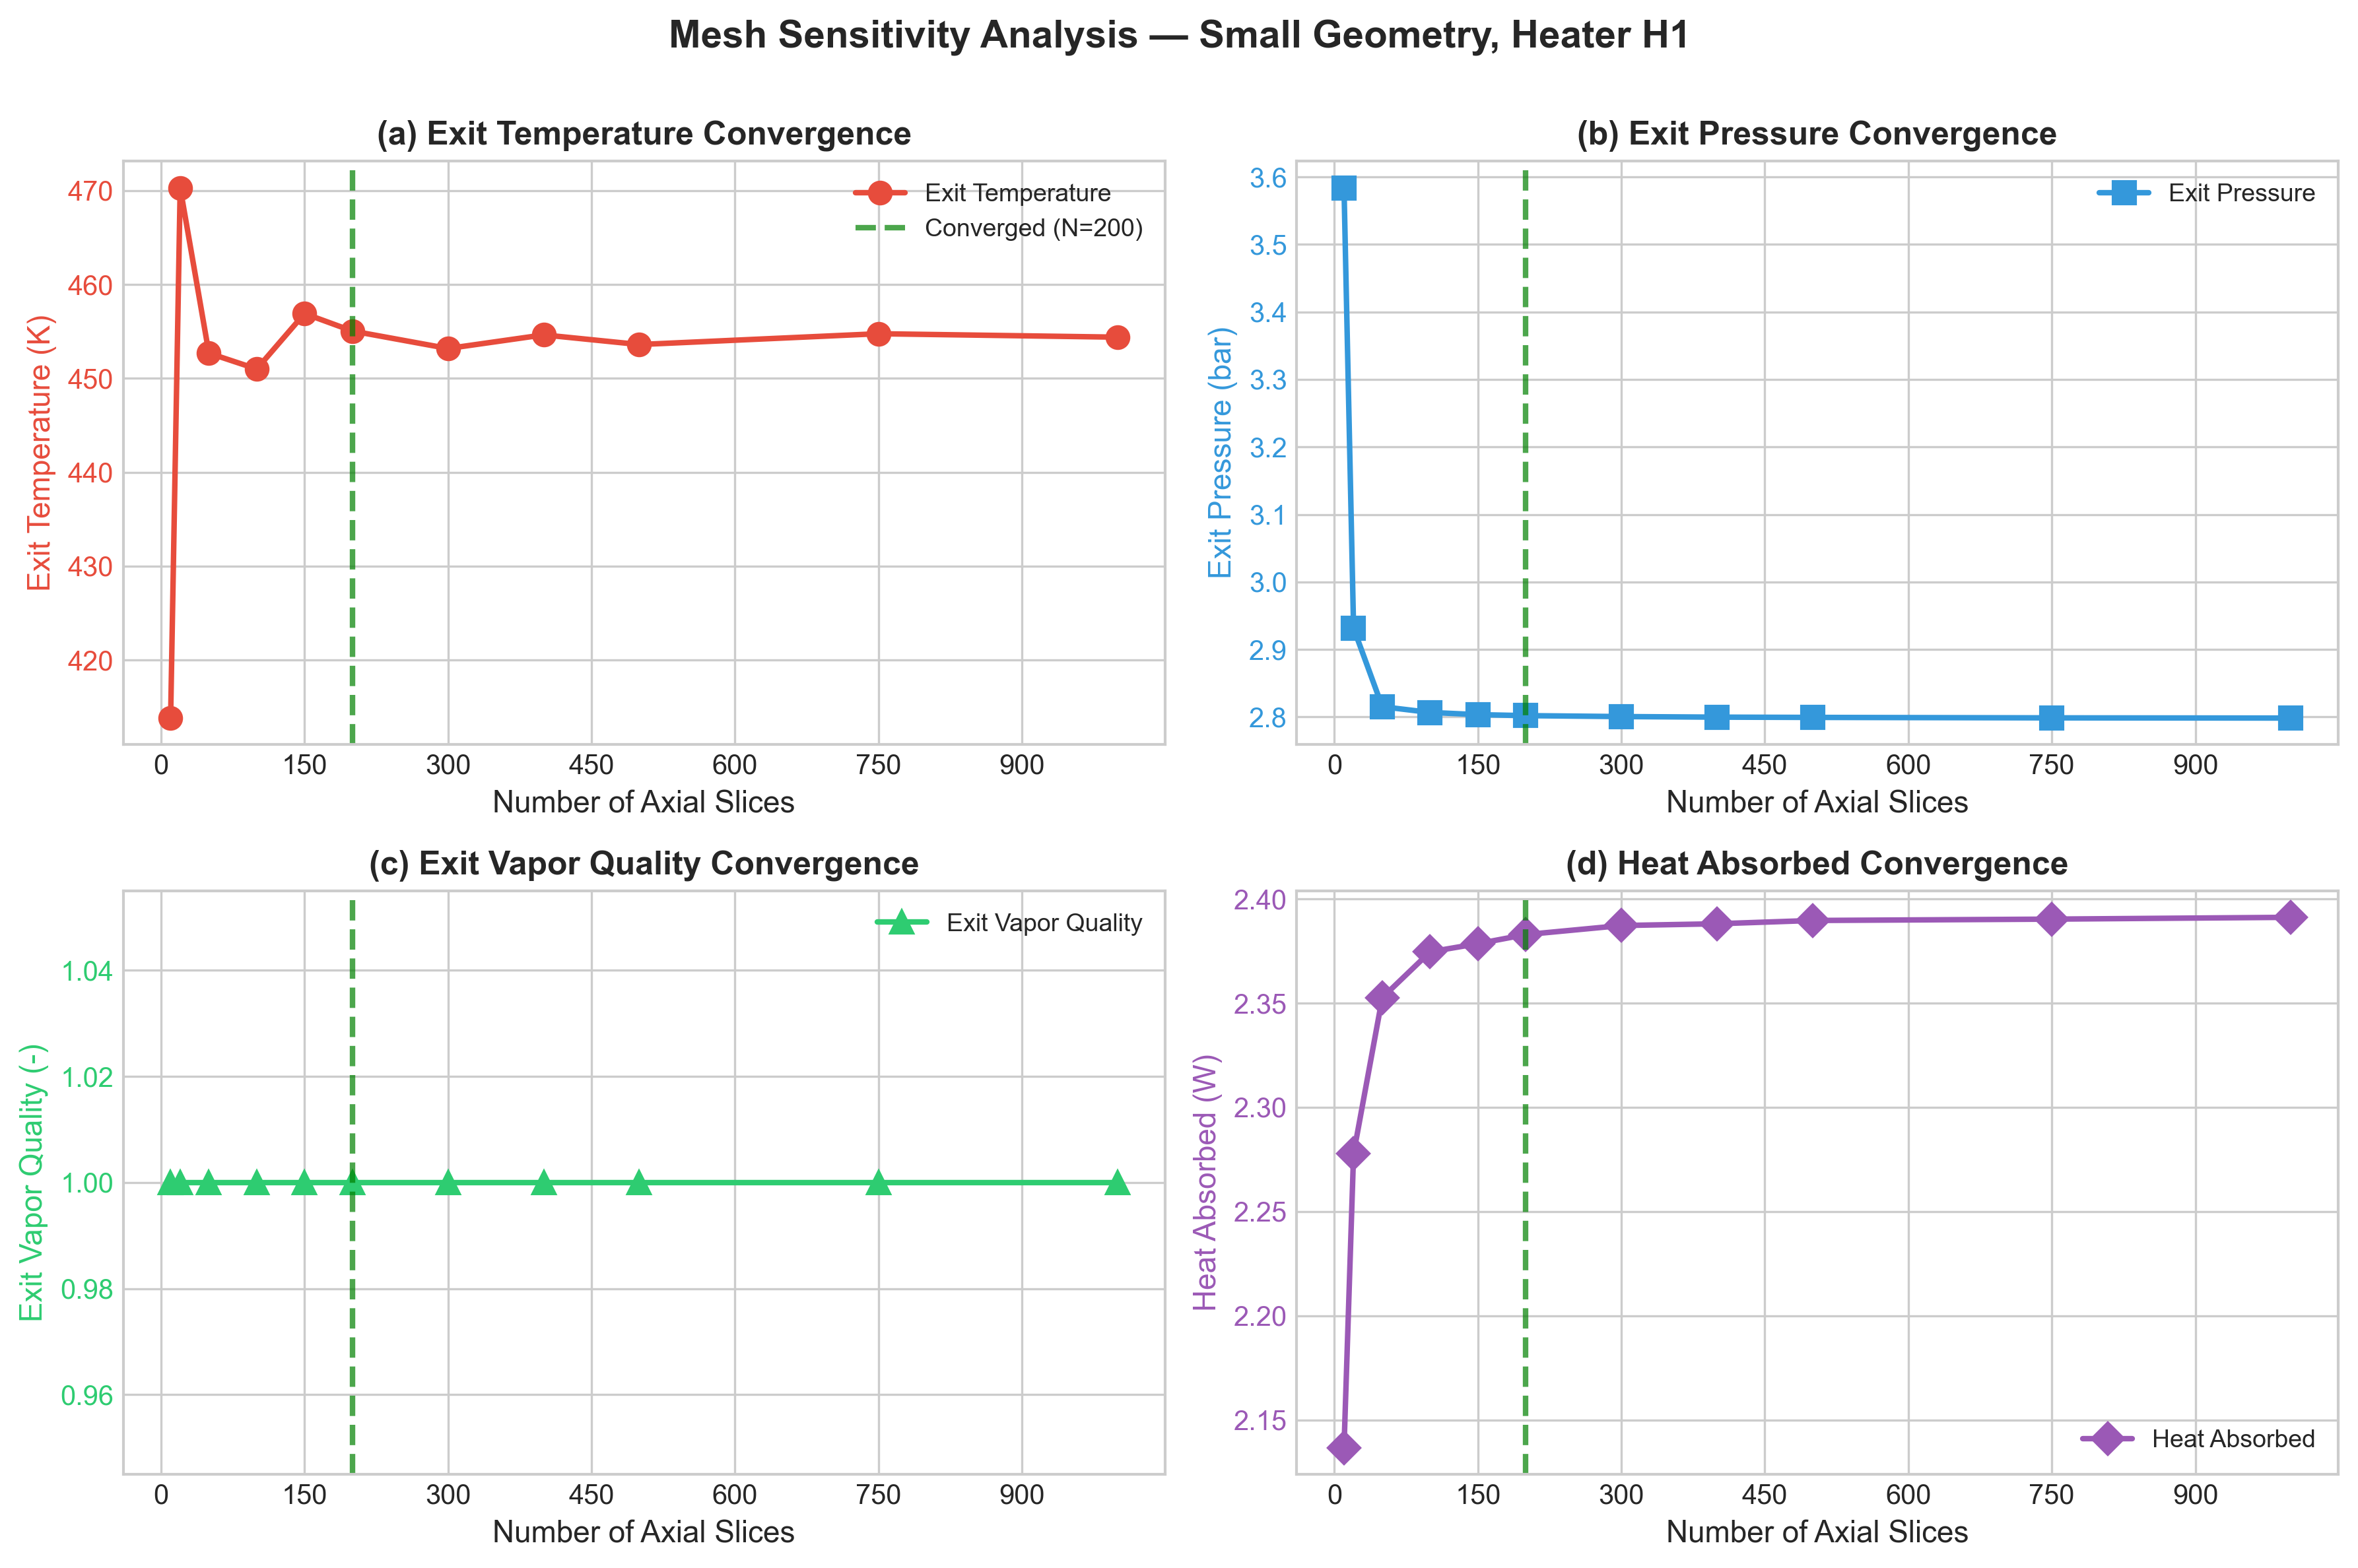
\includegraphics[width=0.9\linewidth]{plots/sensitivity_slices_analysis.png}
  \caption{Mesh-sensitivity analysis for the small geometry (\(w=\SI{40}{\micro m}\)) with heater H1.}
  \label{fig:mesh_sensitivity}
\end{figure}

\subsection*{Geometric parameters (from Silva et al.)}
\begin{tabular}{@{}llll@{}}
\toprule
Item & Symbol & Large case & Small case \\
\midrule
Heater footprint area & \(A_H\) & \(\SI{5.4e-6}{m^2}\) & \(\SI{5.16e-6}{m^2}\) \\
Channel width & \(w\) & \(\SI{212}{\micro m}\) & \(\SI{40}{\micro m}\) \\
Channel depth & \(d\) & \multicolumn{2}{c}{\(\SI{100}{\micro m}\)} \\
Hydraulic diameter & \(D_h\) & derived & derived \\
Channel length & \(L\) & \multicolumn{2}{c}{\(\SI{8.96}{mm}\)} \\
\bottomrule
\end{tabular}

\subsection*{Planar nozzle dimensions (from Silva et al.)}
Widths and divergent lengths (all in \si{\micro m}); discharge coefficients \(C_d\) assigned per type.

\begin{tabular}{@{}lcccccc@{}}
\toprule
Type & \(w_t\) & \(w_{nd}\) & \(l_{nd}\) & \(C_d\) & Exit angle \(\theta\) & Notes \\
\midrule
L & 45 & 500 & 645 & 0.92 & inferred & Longer divergent section \\
W & 45 & 780 & 660 & 0.88 & inferred & Wider, larger angle \\
B & 45 & 500 & 500 & 0.90 & inferred & Short divergent length \\
\bottomrule
\end{tabular}

\subsection*{Material and thermal properties}
Silicon thermal conductivity is modeled as temperature-dependent:


\noindent \(k_{Si}(T)=1.34122\times10^{5} T^{-1.2073}\;\si{W\,m^{-1}\,K^{-1}}\) \cite{SiConductivity}. In the program, this property is calculated at the local wall temperature \(T_w(x)\), and the program iterates until convergence is reached. This ensures that the thermal resistance of the silicon accurately reflects the elevated temperature of the heater stack compared to the fluid. Other properties, including Molybdenum thermal conductivity and heater electrical resistance, are treated as constant values.

\vspace{15pt}


\begin{tabular}{@{}ll@{}}
\toprule
Parameter & Value/Expression \\
\midrule
Silicon nitride conductivity & \(k_{SiN}\approx\SI{3}{W\,m^{-1}K^{-1}}\) \\
SiN thickness & \(t_{SiN}=\SI{500}{nm}\) \\
Silicon conduction thickness & \(t_{Si}=\SI{200}{\micro m}\) \\
TBR (Mo/SiN) & \(R''_{\text{Mo/SiN}}\approx\SI{2e-8}{m^2 K W^{-1}}\) \\
TBR (SiN/Si) & \(R''_{\text{SiN/Si}}\approx\SI{2e-8}{m^2 K W^{-1}}\) \\
Thermal Contact Resistance & \(R''_{\text{TCR}}\approx\SI{1e-4}{m^2 K W^{-1}}\) \\
Heater resistances & \(R_1=\SI{3.40}{\Omega},\;R_2=\SI{2.38}{\Omega}\) \\
\bottomrule
\end{tabular}

\subsection*{Environmental and loss parameters}
\begin{tabular}{@{}ll@{}}
  \toprule
Quantity & Value \\
\midrule
Ambient/base temperature & \(T_\infty=T_{base}=\SI{293.15}{K}\) \\
Surface emissivity & \(\varepsilon=0.8\) \\
\bottomrule
\end{tabular}

\subsection*{Derived relations}
Hydraulic diameter follows \(D_h=4(w d)/(2(w+d))\). Heater power for a selected heater is \(P=V^2/R\).

\section{Boundary conditions and main assumptions}
\begin{tcolorbox}[colback=gray!3!white,colframe=gray!50!black,title=Summary,left=1mm,right=1mm,top=0.6mm,bottom=0.6mm]
Steady, one-dimensional axial march from channel inlet to nozzle entrance. Inlet state is imposed; flow assumed laminar throughout. Two-phase thermodynamics use a homogeneous equilibrium (HEM) mixture with instantaneous saturation at boiling.
\end{tcolorbox}

\subsection*{Mathematical statements}
\begin{description}[leftmargin=3.2cm,labelsep=0.6cm,style=nextline]
  \item[Inlet state]\vspace{-0.3em}
  \[
    T(0)=T_{\text{in}},\qquad p(0)=p_{\text{in}},\qquad \dot m_c=\frac{\dot m_{\text{total}}}{N_{\text{channels}}}.
  \]
  \medskip

  \item[Domain and regime] Steady, 1D axial formulation; laminar flow assumed (validated by resulting \(\mathrm{Re}<2300\)). No turbulent or transitional correlations are invoked.
  \medskip

  \item[Two-phase model]\vspace{-0.3em}
  Homogeneous equilibrium mixture (HEM) with instantaneous saturation in boiling:
  \[
    \rho_m^{-1}=\frac{x}{\rho_v}+\frac{1-x}{\rho_l},\qquad T=\begin{cases}
      T, & x=0,\\[2pt]
      T_{sat}(p), & 0<x<1,\\[2pt]
      T, & x=1.
    \end{cases}
  \]
  
  \begin{tcolorbox}[colback=blue!2!white,colframe=blue!40!black,title=What HEM assumes,left=1mm,right=1mm,top=0.4mm,bottom=0.4mm]
	  	\textit{Homogeneous Equilibrium Model (HEM)} assumes: (i) mechanical equilibrium (common pressure), (ii) thermal equilibrium (common temperature; in boiling the mixture is at \(T_{sat}(p)\)), and (iii) kinematic homogeneity. Mixture density follows \(\rho_m^{-1}=x/\rho_v+(1-x)/\rho_l\); other transport properties use mixing rules.
  \end{tcolorbox}
  \medskip

\end{description}

\section{Channel hydraulics and heat transfer}\label{sec:hydroHT}
\subsection{Flow and friction (laminar regime)}
For a single channel: mean velocity \(u=\dot m_c/(\rho A)\), Reynolds number \(\mathrm{Re}=\rho u D_h/\mu\). Across all simulated cases, the flow remains laminar (\(\mathrm{Re}<2300\)), so we use the laminar smooth-pipe relation
\begin{equation}
  f_s = \frac{64}{\mathrm{Re}}.
\end{equation}
The serpentine friction enhancement \(e_f\) is used. The axial pressure gradient is
\begin{equation}
  \frac{\mathrm{d}p}{\mathrm{d}x} = -\,\frac{f\,\rho u^2}{2 D_h},\qquad f = e_f\,f_s.
\end{equation}
In this formulation, there is no two-phase friction multiplier. While the Homogeneous Equilibrium Model (HEM) captures the pressure drop component due to density reduction and flow acceleration, it neglects the additional dissipation caused by phase interactions (interfacial drag, bubble slip). Consequently, the model likely underestimates the total pressure losses in the boiling region compared to experimental reality.


\subsection{Nusselt number with curvature}
Define Dean number \(\mathrm{De}=\mathrm{Re}\sqrt{D_h/(2R_c)}\). In laminar flow with constant wall heat flux, the baseline is \(\mathrm{Nu}_\ell=4.36\). Curvature enhances mixing; we apply a conservative Dean multiplier consistent with curved-microchannel trends (Rosgueti \emph{et\,al.} \cite{Rosgueti2022}):
\begin{equation}
  e_{De}=1+0.10\,\mathrm{De}^{0.5},\quad 1\le e_{De}\le 3 \;
\end{equation}

The effective Nusselt number is then (with serpentine enhancement factor \(e_{Nu}\) from Rosgueti \emph{et\,al.} \cite{Rosgueti2022})
\begin{equation}
  \mathrm{Nu}= e_{Nu}\,\underbrace{\mathrm{Nu}_\ell}_{4.36}\,e_{De},\qquad 3\le \mathrm{Nu} \le 200,\qquad h=\frac{\mathrm{Nu}\,k}{D_h}.
\end{equation}

\subsection{Heater-to-wall conduction stack}
From the resistive heater to the fluid, heat traverses a series of layers and interfaces modeled as resistances per unit area. With temperature-dependent silicon conductivity \(k_{Si}(T)\), the net series resistance is
\begin{equation}
  R''_\text{stack}=R''_{\text{Mo/SiN}}+\frac{t_{SiN}}{k_{SiN}}+R''_{\text{SiN/Si}}+\frac{t_{Si}}{k_{Si}(T)}+R''_\text{TCR}+R_\text{conv},
\end{equation}
where \(R_\text{conv}=1/\mathcal{H}_c\) is the convective term defined below. The term \(R''_\text{TCR}\) represents the thermal contact resistance due to imperfect contact between layers, which significantly affects thermal conduction. Historically, predicting TCR values is challenging as they can vary widely, typically ranging from \(\SI{5e-6}{m^2 K W^{-1}}\) to \(\SI{5e-4}{m^2 K W^{-1}}\) \cite{cengel2008introduction}. While this value must be correlated with experimental data for this specific case, is essential for accurate simulations. The two thin-film interface resistances (Mo/SiN and SiN/Si) capture thermal boundary resistance (TBR) effects.

\begin{tcolorbox}[colback=gray!5!white,colframe=gray!50!black,title=Conduction path: heater \(\to\) fluid,left=1mm,right=1mm,top=0.5mm,bottom=0.5mm]
Mo/SiN (TBR) \(\to\) SiN film \(\to\) SiN/Si (TBR) \(\to\) bulk Si (\(k_{Si}(T)\)) \(\to\) convection to fluid.
\end{tcolorbox}

\subsection{Wall-to-fluid coupling and wall energy balance}\label{sec:wallbalance}
Per-heater-area convective conductance uses the total wetted perimeter of all channels normalized by heater footprint per unit length \(a'=A_H/L\):
\begin{equation}
  \mathcal{H}_c = h\,\frac{P_{w,\text{tot}}}{a'},\qquad R_\text{conv}=\frac{1}{\mathcal{H}_c}.
\end{equation}
Using \(R''_\text{stack}\) defined above, the wall temperature \(T_w\) solves a per-area steady energy balance
\begin{equation}
  q''_\text{elec} = \underbrace{\frac{T_w-T_f}{R''_\text{stack}}}_{q''_f}+\underbrace{\varepsilon\sigma\,(T_w^4-T_\infty^4)}_{q''_{rad}}+\underbrace{h_{ext}(T_w-T_\infty)}_{q''_{ext}}.
\end{equation}

\section{Nozzle geometry and isentropic model with losses}
\subsection{Planar geometry and discharge angle}
The nozzle is approximated as a rectangular cross-section of depth \(d\). Throat and exit areas are \(A_t=w_t\,d\) and \(A_e=w_{nd}\,d\). The planar divergence half-angle is
\begin{equation}
  \theta = \arctan\!\left(\frac{w_{nd}-w_t}{2\,l_{nd}}\right),
\end{equation}
which causes an axial thrust projection factor \(\lambda_{\text{planar}} = \frac{\sin \theta}{\theta}\).

\subsection{Isentropic relations and discharge coefficient}
Assuming ideal-gas isentropic expansion with ratio of specific heats \(\gamma\) and gas constant \(R\), the area--Mach relation gives the supersonic exit Mach number \(M_e\) from \(A_e/A_t\). The choked (sonic) mass flow at the throat, including a discharge coefficient \(C_d\in(0,1)\), is
\begin{equation}
  \dot m_* = C_d\,\frac{A_t\,p_0\,\gamma\,\sqrt{\left(\tfrac{2}{\gamma+1}\right)^{\tfrac{\gamma+1}{\gamma-1}}}}{\sqrt{\gamma\,R\,T_0}}.
\end{equation}
Given \(M_e\), exit temperature and pressure are
\begin{equation}
  T_e = \frac{T_0}{1+\tfrac{\gamma-1}{2}M_e^2},\qquad p_e = p_0\left(1+\tfrac{\gamma-1}{2}M_e^2\right)^{-\tfrac{\gamma}{\gamma-1}},
\end{equation}
with exhaust speed \(V_e=M_e\sqrt{\gamma R T_e}\). The model limits the nozzle mass flow to the smaller of the choked capacity and the available vapor mass flow \(\dot m_v=x_{\text{exit}}\,\dot m_{\text{total}}\). The thrust and specific impulse (projected axially) are
\begin{equation}
  F=\dot m\,V_e\,\lambda_{\text{planar}} + (p_e-p_a)A_e,\qquad I_{sp}=\frac{F}{\dot m\,g_0}.
\end{equation}
Lower \(C_d\) captures viscous, non-ideal, and end effects; a larger \(\theta\) reduces the axial momentum component via \(\lambda_{\text{planar}}\). Nozzle widths and divergent lengths used to infer \(\theta\) are taken from Silva \emph{et\,al.} \cite{Silva2023}.

\section{Results overview}
Table~\ref{tab:summary} lists the 12 modeled cases across heaters (H1, H2), geometries (Large/Small), and nozzle types (L, W, B). The final values for thrust and specific impulse are feasible.

\begin{table}[h]
  \centering
  \small
  \caption{Compact results summary (selected columns).}
  \label{tab:summary}
  \begin{tabular}{@{}rrrrrrrrrrr@{}}
    \toprule
    Case & Ht & Geom & Noz & $P$ [W] & $Q$ [W] & Util & $\dot m_N$ [mg/s] & $F$ [mN] & $I_{sp}$ [s] \\
    \midrule
    1 & H1 & Large & L & 7.4 & 2.19 & 0.30 & 0.78 & 0.96 & 126.0 \\
    2 & H1 & Large & W & 7.4 & 2.19 & 0.30 & 0.78 & 0.89 & 117.2 \\
    3 & H1 & Large & B & 7.4 & 2.19 & 0.30 & 0.78 & 0.93 & 122.4 \\
    4 & H1 & Small & L & 7.4 & 2.62 & 0.36 & 0.28 & 0.33 & 121.3 \\
    5 & H1 & Small & W & 7.4 & 2.62 & 0.36 & 0.27 & 0.30 & 115.1 \\
    6 & H1 & Small & B & 7.4 & 2.62 & 0.36 & 0.27 & 0.31 & 117.4 \\
    7 & H2 & Large & L & 10.5 & 2.73 & 0.26 & 0.82 & 1.22 & 151.2 \\
    8 & H2 & Large & W & 10.5 & 2.73 & 0.26 & 0.82 & 1.14 & 141.4 \\
    9 & H2 & Large & B & 10.5 & 2.73 & 0.26 & 0.82 & 1.18 & 146.8 \\
    10 & H2 & Small & L & 10.5 & 2.90 & 0.28 & 0.24 & 0.33 & 138.6 \\
    11 & H2 & Small & W & 10.5 & 2.90 & 0.28 & 0.23 & 0.30 & 131.6 \\
    12 & H2 & Small & B & 10.5 & 2.90 & 0.28 & 0.24 & 0.31 & 134.2 \\
    \bottomrule
  \end{tabular}
\end{table}


\subsection*{Pressure and temperature distributions along the heating chamber.}

The plots show axial profiles of temperature, pressure, and quality.

\paragraph{Case 1 (H1, Large geometry).}
Temperature rises from the inlet until the local saturation temperature is reached. Upon the onset of boiling, the fluid temperature pins to \(T_{sat}(p)\) while added heat goes into latent energy. The profile stays at saturation nearly to the exit because not all of the liquid is vaporized; the predicted exit quality is \(x\approx 0.945\). A subtle kink in the pressure trace appears when it starts boiling. Physically, the onset of vapor formation reduces the mixture density and increases velocity. This acceleration raises the frictional pressure gradient \(|\mathrm{d}p/\mathrm{d}x|\), so the pressure drops slightly faster immediately after boiling begins.


\begin{figure}[h]
  \centering
  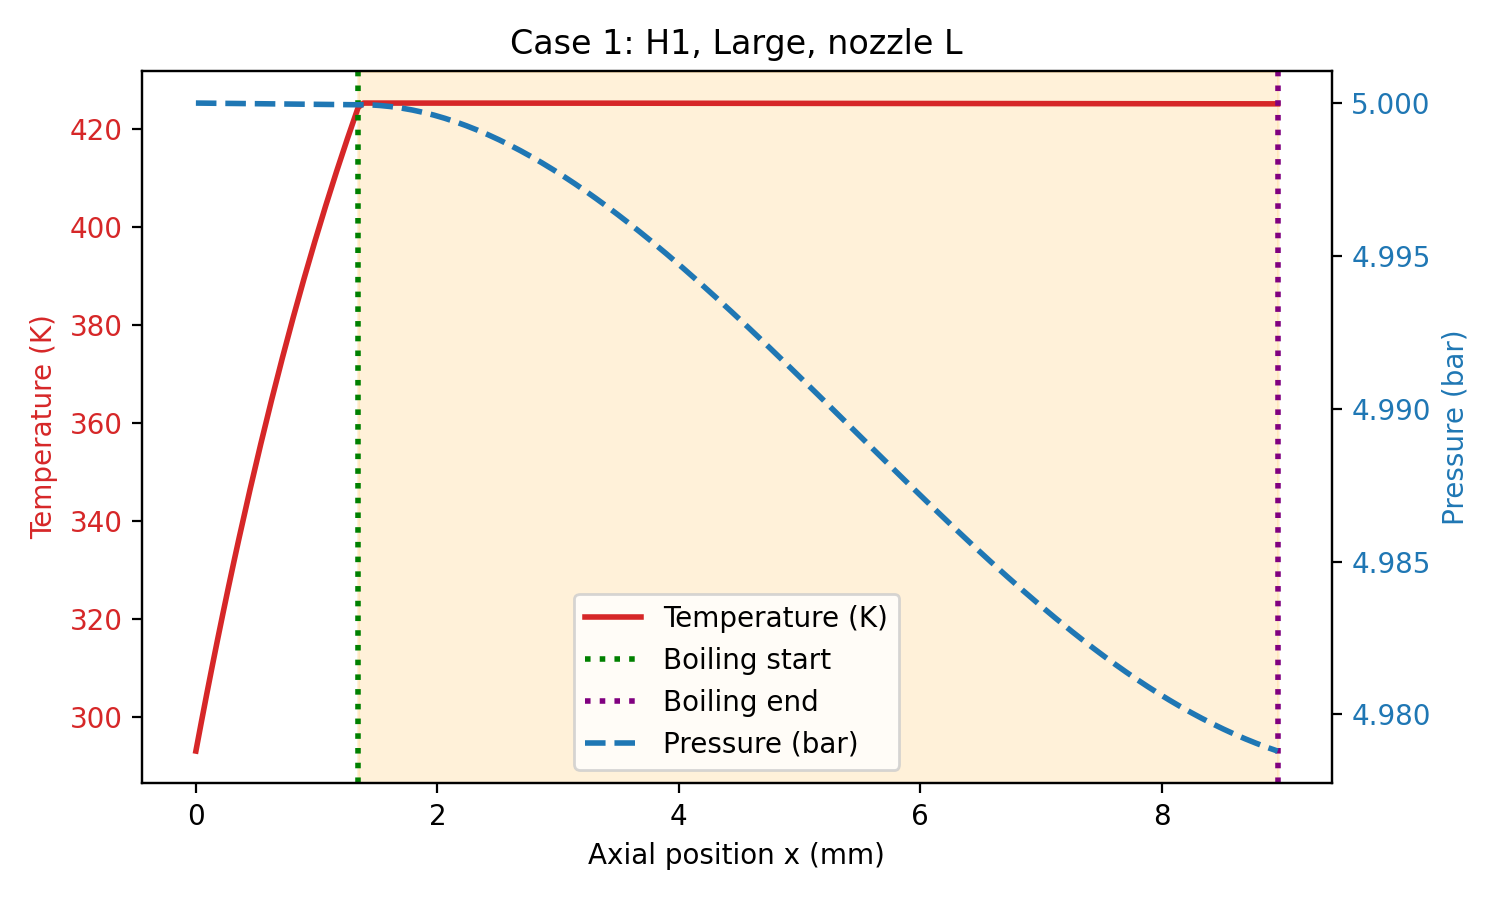
\includegraphics[width=0.7\linewidth]{plots/case_01_H1_Large_L.png}
  \caption{Case 1 (H1, Large geometry). Temperature rises to saturation and remains at \(T_{sat}(p)\) while boiling proceeds; exit quality is \(x\approx0.945\). A mild increase in pressure gradient appears at boiling onset due to decreasing density and increasing two-phase friction.}
  \label{fig:case1}
\end{figure}

\FloatBarrier

\paragraph{Case 4 (H1, Small geometry).}
The temperature increases to \(T_{sat}(p)\), after which a pronounced pressure drop occurs. This steep decline is much stronger than in Case 1 because the small geometry has a much smaller hydraulic diameter \(D_h\), yielding larger friction losses via
\(\mathrm{d}p/\mathrm{d}x\propto f\,\rho u^2/(2D_h)\). With the same per-channel mass flow on a smaller cross-section, velocity and dynamic pressure are higher, and once boiling begins the rapid density reduction further accelerates the flow. As pressure plummets, the saturation temperature drops with \(p\), so the fluid temperature also decreases while boiling continues. When the liquid fully vaporizes (\(x\to 1\)), sensible heating resumes and the vapor temperature rises again toward the exit.


\begin{figure}[h]
  \centering
  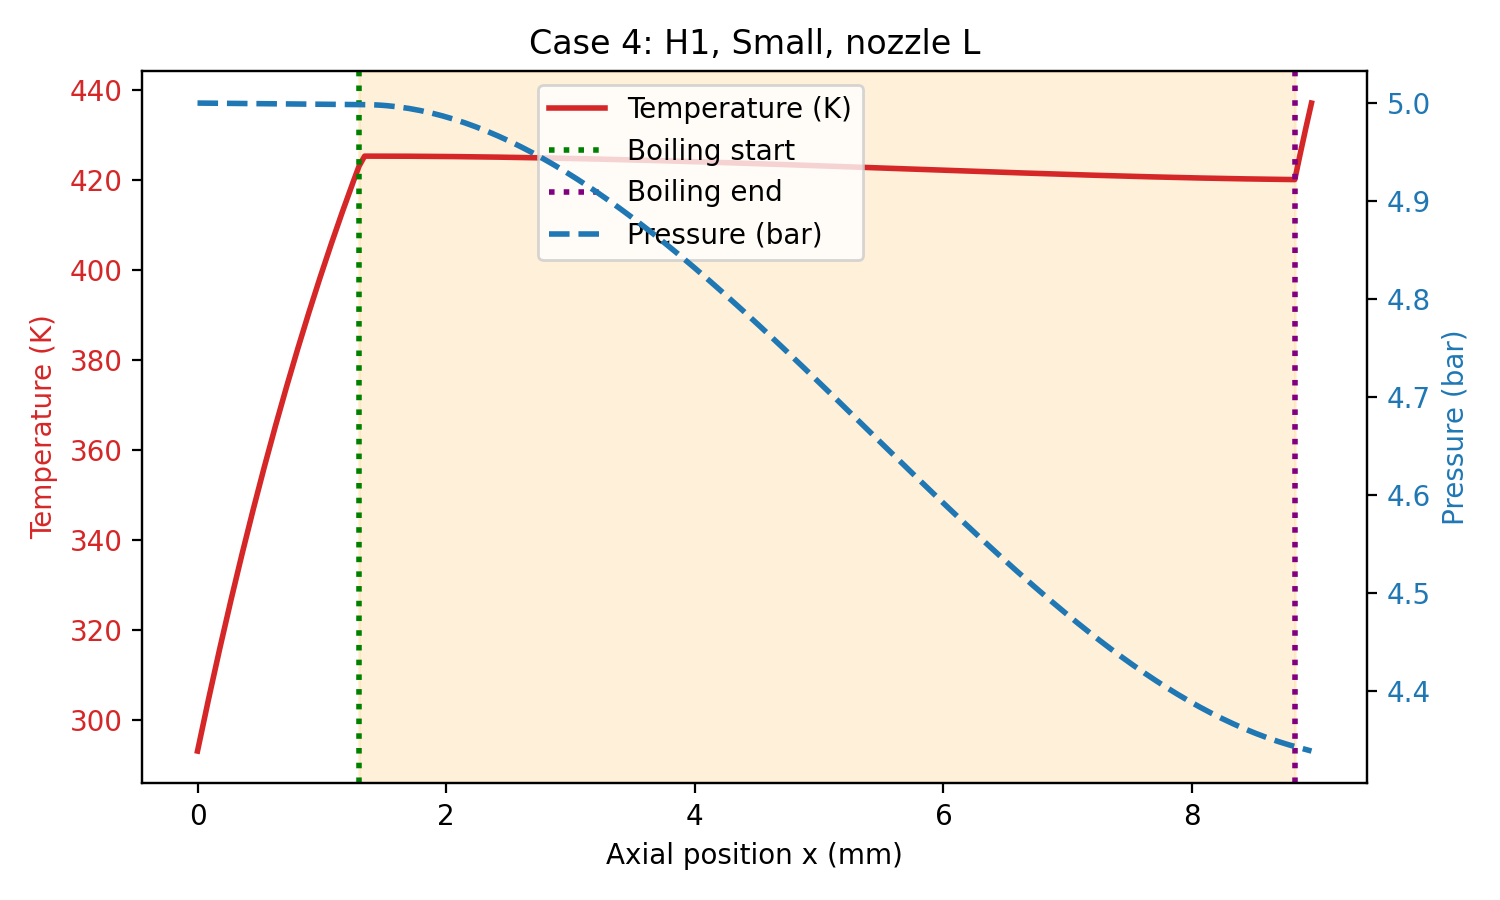
\includegraphics[width=0.7\linewidth]{plots/case_04_H1_Small_L.png}
  \caption{Case 4 (H1, Small geometry). A pronounced two-phase pressure drop develops after boiling onset because the smaller hydraulic diameter raises friction losses and velocity; \(T_{sat}(p)\) falls with pressure, producing a temporary temperature decrease until complete vaporization.}
  \label{fig:case4}
\end{figure}

\FloatBarrier

\paragraph{Case 7 (H2, Large geometry).}
This case mirrors the qualitative behavior of Case 1 but with higher electrical power. The added power vaporizes the flow well before the exit, leaving a longer downstream length for superheating the vapor. Consequently, exit vapor temperature and thrust increase relative to Case 1.


\begin{figure}[h]
  \centering
  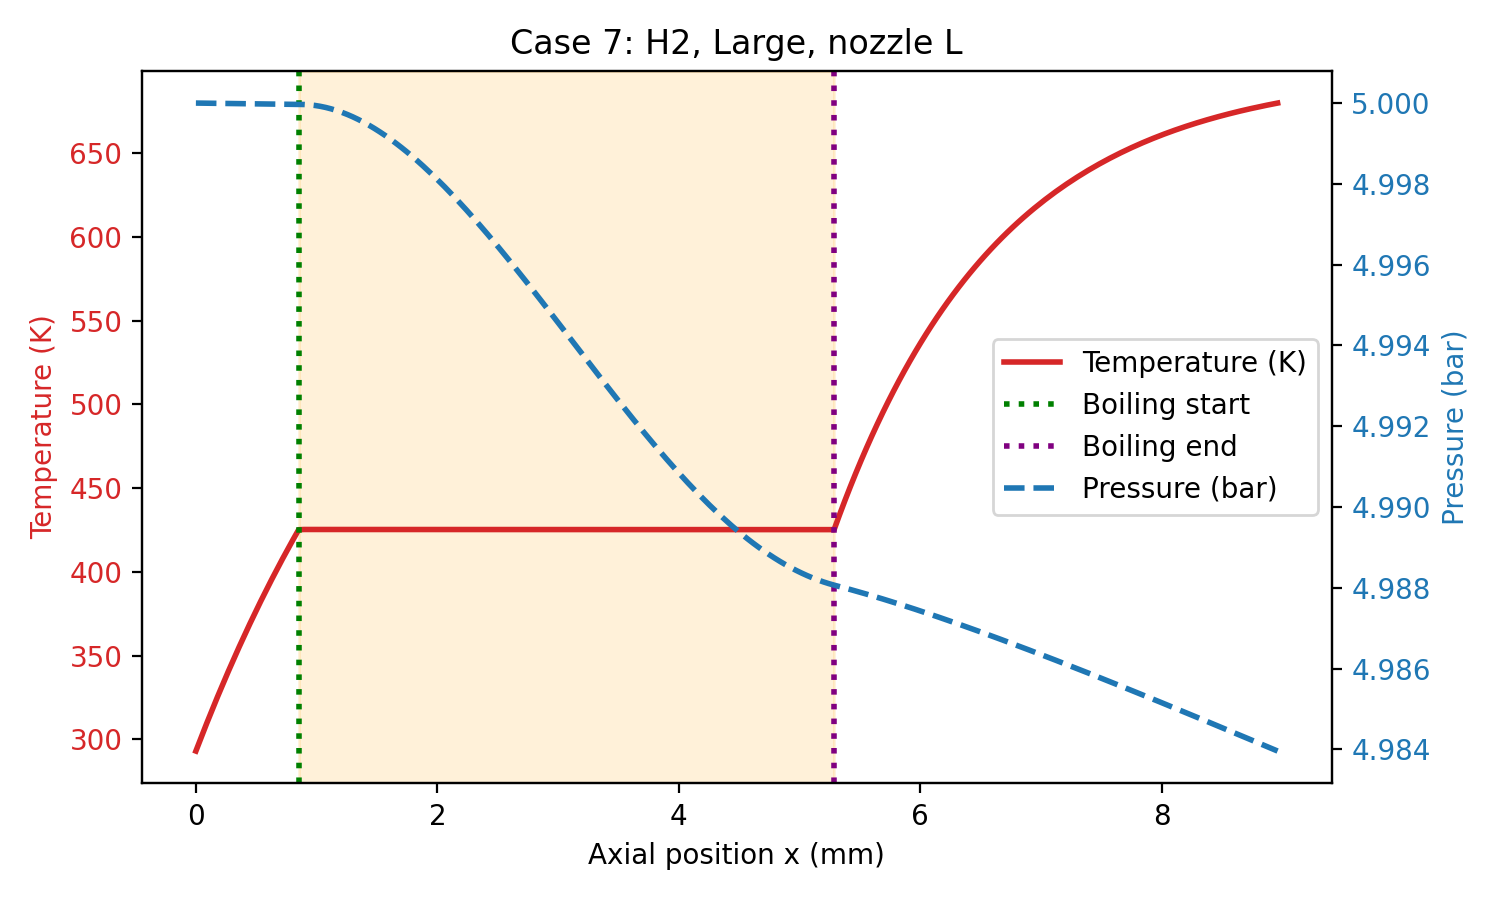
\includegraphics[width=0.7\linewidth]{plots/case_07_H2_Large_L.png}
  \caption{Case 7 (H2, Large geometry). Higher power drives complete boiling well upstream of the exit, leaving more length to superheat the vapor.}
  \label{fig:case7}
\end{figure}

\FloatBarrier

\paragraph{Case 10 (H2, Small geometry).}
The evolution resembles Case 4 (same small geometry), including the strong depressurization through the boiling region. The higher power drives the system to a higher final temperature after complete vaporization, but the unrealistic magnitude of the pressure drop persists.


\begin{figure}[h]
  \centering
  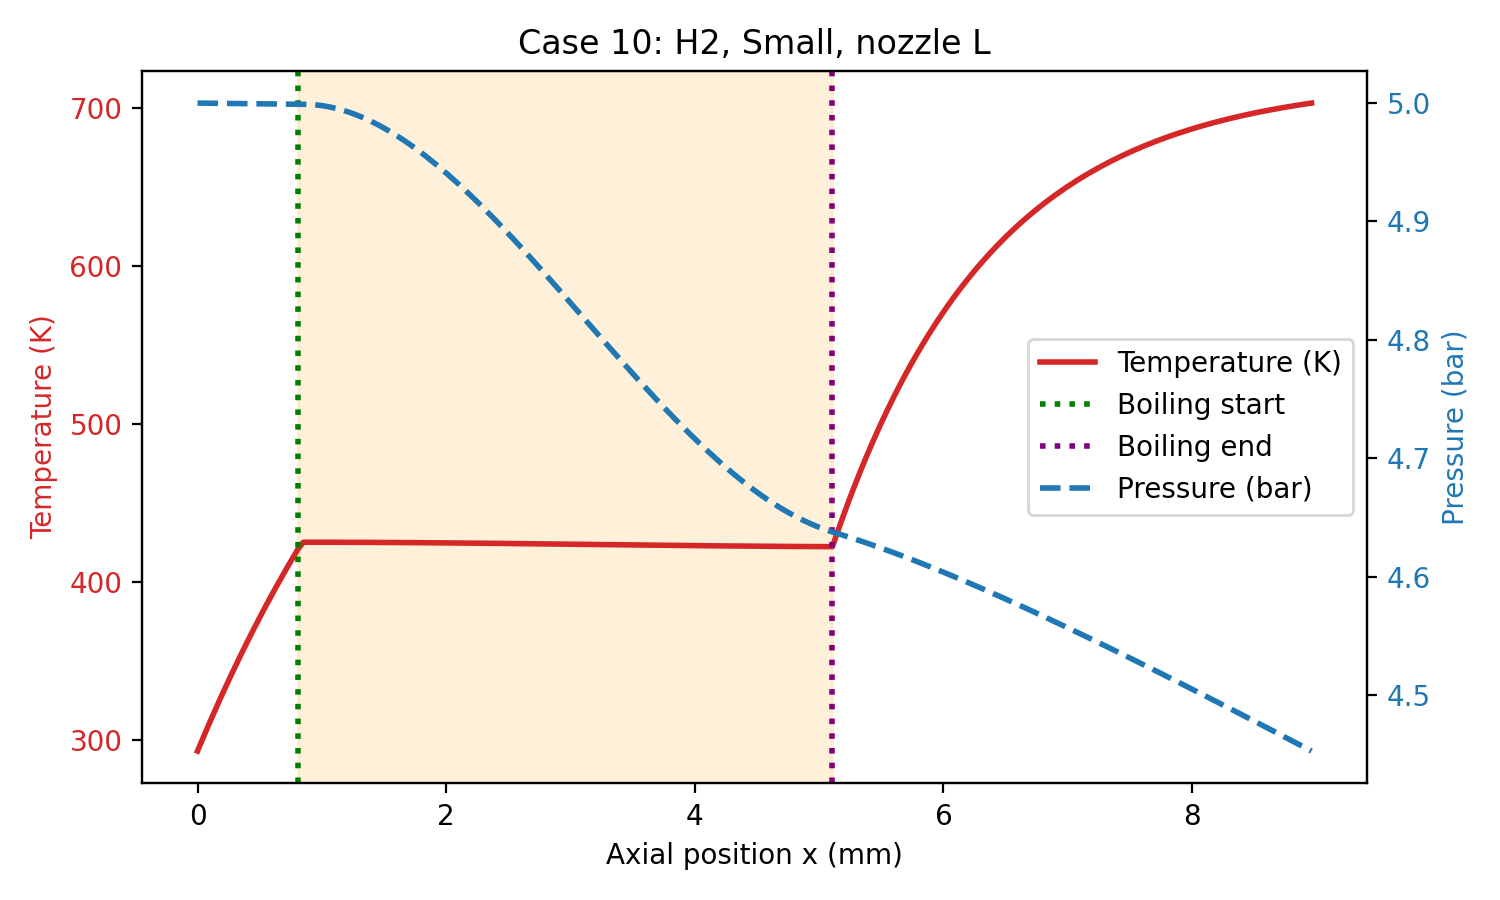
\includegraphics[width=0.7\linewidth]{plots/case_10_H2_Small_L.png}
  \caption{Case 10 (H2, Small geometry). Similar to Case 4 with strong depressurization through boiling; higher power yields a higher final vapor temperature by the exit.}
  \label{fig:case10}
\end{figure}

\FloatBarrier

\begin{tcolorbox}[colback=yellow!6!white,colframe=yellow!40!black,title=Interpretation and model limitation,left=1mm,right=1mm,top=0.6mm,bottom=0.6mm]
For the small-geometry cases, the steep depressurization indicates that the present friction model likely overpredicts two-phase pressure losses at these scales. It performs reasonably for the larger geometry but appears to “break” for the smaller one, leading to exit pressures that are not physically plausible and to the non-monotone temperature behavior tied to \(T_{sat}(p)\). Addressing this requires a microchannel-specific two-phase pressure-drop correlation.
\end{tcolorbox}


\section{Conclusions}

\subsection*{Answer to the research questions}
	extbf{RQ1.} A concise, traceable model for these VLM geometries is a 1D laminar axial march with Dean-number curvature enhancements for friction and heat transfer, a homogeneous equilibrium (HEM) two-phase treatment (temperature locked to saturation during boiling), a multilayer wall conduction balance (heater/TBR/SiN/Si + radiation + external convection), and an isentropic planar nozzle with a discharge coefficient and axial projection. This set captures the main coupled phenomena (heating, boiling onset, latent absorption, superheating) with limited computational cost.

	extbf{RQ2.} Large channels show moderate pressure decline and a stable saturation plateau; increasing power moves complete vaporization upstream and allows downstream superheating (raising thrust and \(I_{sp}\)). Small channels display very steep pressure drops during boiling and a temporary temperature dip as falling pressure lowers \(T_{sat}\); this likely reflects friction overprediction, not true device behavior. Representative thrust lies around \(0.9{-}1.2\,\text{mN}\) for large geometry and somewhat lower for small; specific impulse reaches \(\sim 150\,\text{s}\) at higher power.

\subsection*{Key observations}
\begin{itemize}[nosep]
  \item Boiling onset produces a sharper pressure gradient via density reduction and flow acceleration.
  \item Higher heater power (H2) shifts complete vaporization upstream, enabling vapor superheat and higher performance.
  \item Small geometry predictions show unrealistically deep depressurization, flagging the need for better two-phase friction correlations.
  \item Exit quality near unity is only achieved early enough for superheating at higher power and/or larger hydraulic diameter.
\end{itemize}

\subsection*{Main limitations and next steps}
\begin{itemize}[nosep]
  \item HEM (no slip) without a dedicated two-phase friction multiplier likely underpredicts pressure drop in the boiling region.
  \item CHF not modeled; high-flux stability margins remain unknown.
  \item Curvature/boiling heat-transfer enhancements are heuristic bounds, not dimension-specific correlations.
  \item Nozzle model ignores detailed viscous and non-equilibrium effects.
\end{itemize}
Priority improvements: integrate microchannel boiling pressure-drop correlations including slip, add nucleate/film boiling heat-transfer regimes and CHF criteria, and validate against measured axial temperature/pressure using heater sensing.



\bibliographystyle{ieeetr}
\bibliography{references}

\end{document}
